
%%%%%%%%%%%%%%%%%%%%%%%%%%%%%%%%%%%%%%%%%%%%%%%%%%%%%%%%
%
% Copyright (c) 2003-2010 by University of Queensland
% Earth Systems Science Computational Center (ESSCC)
% http://www.uq.edu.au/esscc
%
% Primary Business: Queensland, Australia
% Licensed under the Open Software License version 3.0
% http://www.opensource.org/licenses/osl-3.0.php
%
%%%%%%%%%%%%%%%%%%%%%%%%%%%%%%%%%%%%%%%%%%%%%%%%%%%%%%%%

In this chapter we will investigate the effects of a current flow and
resistivity in a medium. This type of problem is related to the DC resistivity method of
geophysical prospecting. Currents are injected into the ground at the surface
and measurements of the potential are taken at various potential-dipole
locations along or adjacent to the survey line. From these measurements of the
potential it is possible to infer an approximate apparent resistivity model of
the subsurface.

The following theory comes from a tutorial by \citet{Loke2004}.
We know from Ohm's law that the current flow in the ground is given in vector
form by
\begin{equation}
\vec{J}=\sigma\vec{E}
\end{equation}
where $\vec{J}$ is current density, $\vec{E}$ is the electric field intensity
and $\sigma$ is the conductivity. We can relate the potential to the electric
field intensity by 
\begin{equation}
E=-\nabla\Phi
\end{equation}
where $\Phi$ is the potential. We now note that the current density is related
to the potential via
\begin{equation}
\vec{J}=-\sigma\nabla\Phi
\end{equation}
Geophysical surveys predominantly use current sources which individually act as
point poles. Considering our model will contain volumes, we can normalise the
input current and approximate the current density in a volume $\Delta V$ by
\begin{equation}
\nabla \vec{J} =
\left(\frac{I}{\Delta V} \right) \delta(x-x_{s})
								 \delta(y-y_{s})
								 \delta(z-z_{s})
\end{equation}

\begin{equation}
-\nabla \cdot \left[ \sigma(x,y,z) \nabla \phi (x,y,z) \right] =
\left(\frac{I}{\Delta V} \right) \delta(x-x_{s})
								 \delta(y-y_{s})
								 \delta(z-z_{s})			 
\end{equation}

This form is quite simple to solve in \esc.

\section{3D Current-Dipole Potential}
\sslist{example11m.py; example11c.py}

\begin{figure}[ht]
\centering
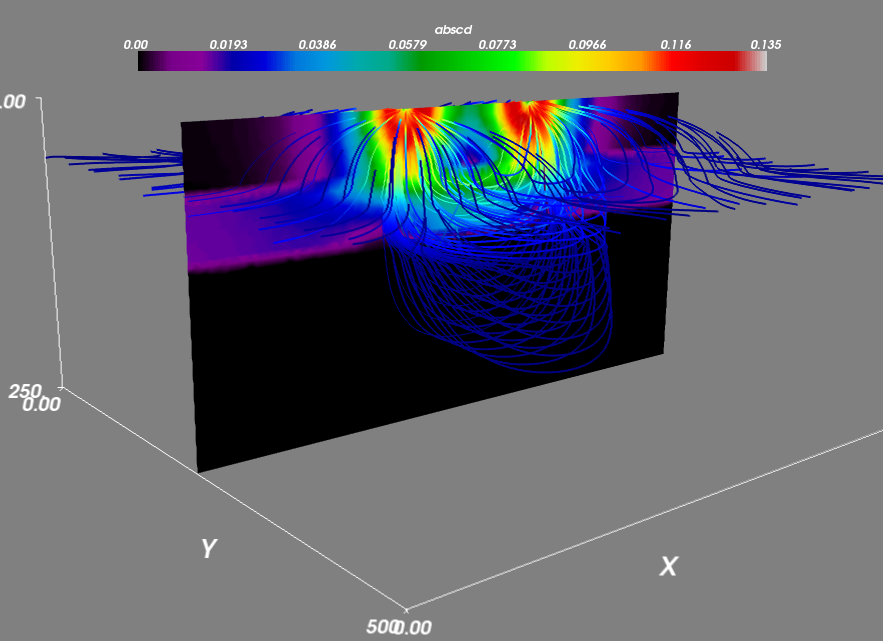
\includegraphics[width=0.95\textwidth]{figures/ex11cstreamline.png}
\caption{Current Density Model for layered medium.}
\label{fig:ex11cstream}
\end{figure}

\section{Frequency Dependent Resistivity - Induced Polarisation}
With a more complicated resistivity model it is possible to calculate the
chargeability or IP effect in the model. A recent development has been the
Fractal model for complex resistivity \citep{Farias2010,Honig2007}.


The model is calculated over many frequencyies and transformed to the time
domain using a discrete fourier transform.

